
  
\DocumentMetadata{
 lang=en,
 pdfversion=2.0,
 pdfstandard=ua-2,
 pdfstandard=a-4,
 testphase=
   {
    phase-III, %lists,footnotes,sectioning,
               %toc,marginpar,bibliography,floats,
               %graphics ...
    table, %tabular, tabularx, longtable
    title  %maketitle
   },
 lang=de-DE  
 }
\AddToHookWithArguments{env/otherlanguage/begin}{\tagpdfsetup{text/lang=\BCPdata{language}}} 
  \documentclass[a4paper,12pt]{article}
  \usepackage[english,ngerman]{babel}
  \usepackage{graphicx}
  \usepackage[hidelinks]{hyperref}
  \usepackage[left=1.1cm,right=1.1cm]{geometry}
  \setlength\leftmargini{5.7cm}
  \usepackage{fontspec}
  % https://fonts.google.com/specimen/Almendra
  \setmainfont[BoldFont=Almendra-Bold.ttf]{Almendra-Regular.ttf}
  \makeatletter
  \renewcommand\section{\@startsection {section}{1}{\z@}%
                                   {-3.5ex \@plus -1ex \@minus -.2ex}%
                                   {2.3ex \@plus.2ex}%
                                   {\centering\normalfont\LARGE\bfseries}}
  \makeatother
  \setcounter{secnumdepth}{-1}  
  \begin{document}
  
  
\begin{otherlanguage}{english}

  \section[Max und Moritz]{The Project Gutenberg eBook of {Max und
      Moritz: Eine Bubengeschichte in sieben
      Streichen}\label{pg-header-heading}}

    


This ebook is for the use of anyone anywhere in the United States and
most other parts of the world at no cost and with almost no restrictions
whatsoever. You may copy it, give it away or re-use it under the terms
of the Project Gutenberg License included with this ebook or online
at \href{https://www.gutenberg.org}{www.gutenberg.org}. If you are not located in the United States,
you will have to check the laws of the country where you are located
before using this eBook.

    
\end{otherlanguage}


\bigskip

\textbf{Title}: Max und Moritz: Eine Bubengeschichte in sieben Streichen

\textbf{Author}: Wilhelm Busch


\smallskip

\begin{otherlanguage}{english}
\textbf{Release date}: November 26, 2005 [eBook \#17161]

                Most recently updated: December 13, 2020

        Converted to \textsf{\LaTeX} to produce Tagged PDF, \textsf{\LaTeX} Project, March 2024

\smallskip
                
\textbf{Language}: German

\smallskip
                
\textbf{Credits}: Produced by Inka Weide, Robert Kropf, Markus Brenner and
        the Online Distributed Proofreading Team at
        \url{https://www.pgdp.net}


\smallskip

\textbf{Transcriber's notes}: 
``Düte'', ``Zippelmütze'' sind alte Wortformen / are old spelled words
\end{otherlanguage}


\bigskip
\hrule

\clearpage


\title{Max und Moritz}
\author{Wilhelm Busch}
\maketitle


\begin{center}
eine\\
Bubengeschichte\\
in\\
sieben Streichen  
\end{center}

\begin{center}
von
\end{center}

\begin{center}
Wilhelm Busch.  
\end{center}


\begin{center}
Dreiundfünfzigste Auflage\\
1906 
\end{center}



\begin{center}
München\\
Verlag von Braun und Schneider.
\end{center}




\begin{center}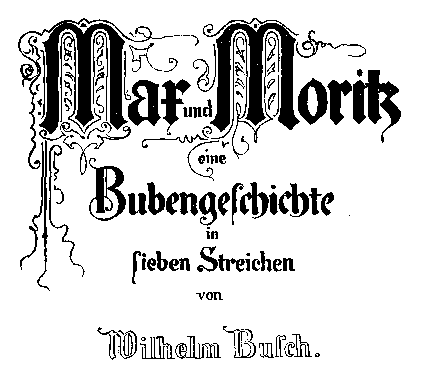
\includegraphics[scale=.7, alt={Titelblatt}]{images/titel.png}\end{center}


\bigskip
\hrule

\clearpage
\tableofcontents


\bigskip
\hrule

\clearpage
\section{Vorwort.\label{Vorwort}}


\begin{verse}
Ach, was muß man oft von bösen\\{}
Kindern hören oder lesen!\\{}
Wie zum Beispiel hier von diesen,
\end{verse}



\begin{center}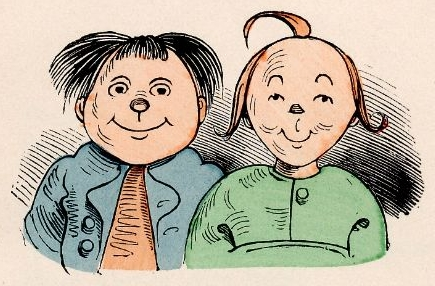
\includegraphics[scale=.7, alt={Max und Moritz}]{images/0-01.jpg}\end{center}



\begin{verse}
Welche Max und Moritz hießen.\\{}
Die, anstatt durch weise Lehren\\{}
Sich zum Guten zu bekehren,\\{}
Oftmals noch darüber lachten\\{}
Und sich heimlich lustig machten.~—\\{}
— Ja, zur Übeltätigkeit,\\{}
Ja, dazu ist man bereit!~—\\{}
— Menschen necken, Tiere quälen,\\{}
Äpfel, Birnen, Zwetschgen stehlen~—\\{}
Das ist freilich angenehmer\\{}
Und dazu auch viel bequemer,\\{}
Als in Kirche oder Schule\\{}
Festzusitzen auf dem Stuhle.~—\\{}
— Aber wehe, wehe, wehe!\\{}
Wenn ich auf das Ende sehe!!~—\\{}
— Ach, das war ein schlimmes Ding,\\{}
Wie es Max und Moritz ging.\\{}
— Drum ist hier, was sie getrieben,\\{}
Abgemalt und aufgeschrieben.
\end{verse}


\hrule


\clearpage
\section{Erster Streich.\label{Erster_Streich}}


\begin{verse}
Mancher gibt sich viele Müh'\\{}
Mit dem lieben Federvieh;\\{}
Einesteils der Eier wegen,\\{}
Welche diese Vögel legen,\\{}
Zweitens: Weil man dann und wann\\{}
Einen Braten essen kann;\\{}
Drittens aber nimmt man auch\\{}
Ihre Federn zum Gebrauch\\{}
In die Kissen und die Pfühle,\\{}
Denn man liegt nicht gerne kühle.~—
\end{verse}



\begin{center}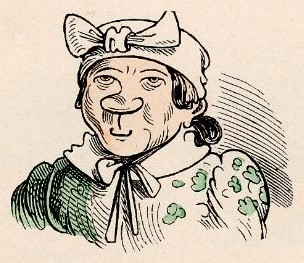
\includegraphics[scale=.7, alt={Witwe Bolte}]{images/1-01.jpg}\end{center}



\begin{verse}
Seht, da ist die Witwe Bolte,\\{}
Die das auch nicht gerne wollte.
\end{verse}



\begin{center}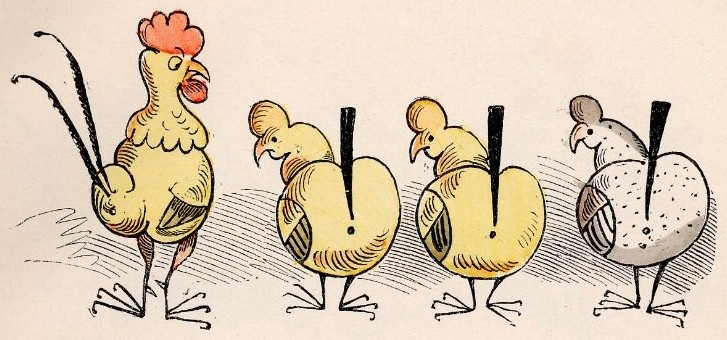
\includegraphics[scale=.7, alt={Drei Hühner und ein Hahn}]{images/1-02.jpg}\end{center}



\begin{verse}
Ihrer Hühner waren drei\\{}
Und ein stolzer Hahn dabei.~—\\{}
Max und Moritz dachten nun:\\{}
Was ist hier jetzt wohl zu tun?~—\\{}
— Ganz geschwinde, eins, zwei, drei\\{}
Schneiden sie sich Brot entzwei,\\{}
In vier Teile jedes Stück\\{}
Wie ein kleiner Finger dick.\\{}
Diese binden sie an Fäden,\\{}
Übers Kreuz, ein Stück an jeden,
\end{verse}



\begin{center}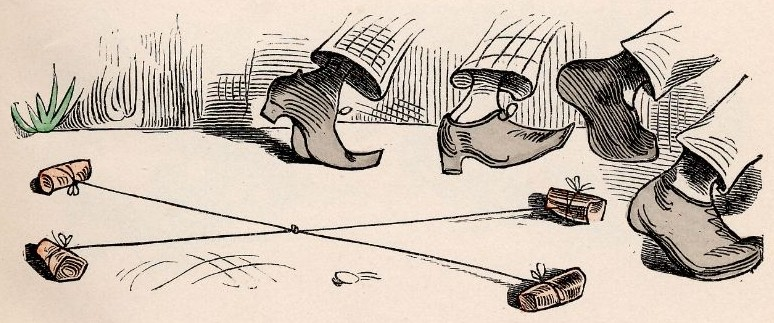
\includegraphics[scale=.7, alt={Vier Brotstücke}]{images/1-03.jpg}\end{center}



\begin{verse}
Und verlegen sie genau\\{}
In den Hof der guten Frau.~—
\end{verse}



\begin{center}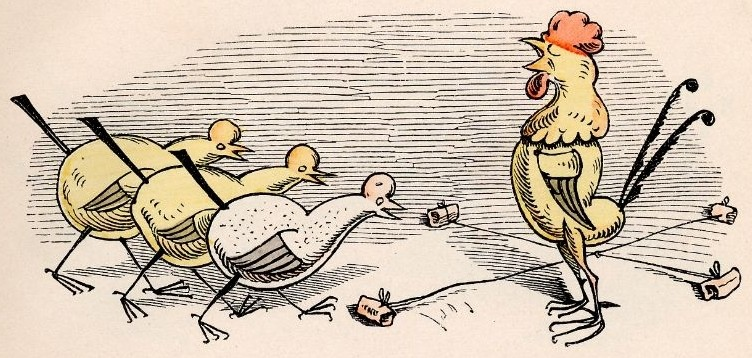
\includegraphics[scale=.7, alt={Da kommen sie}]{images/1-04.jpg}\end{center}



\begin{verse}
Kaum hat dies der Hahn gesehen,\\{}
Fängt er auch schon an zu krähen:\\{}
Kikeriki! Kikikerikih!!\\{}
Tak, tak, tak!~— da kommen sie.
\end{verse}



\begin{center}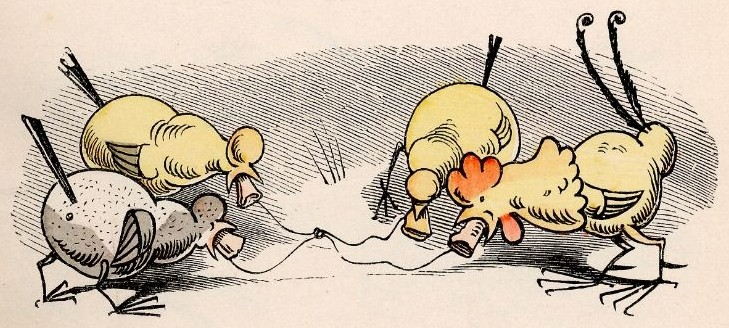
\includegraphics[scale=.7, alt={... und schlucken das Brot}]{images/1-05.jpg}\end{center}



\begin{verse}
Hahn und Hühner schlucken munter\\{}
Jedes ein Stück Brot hinunter;
\end{verse}



\begin{center}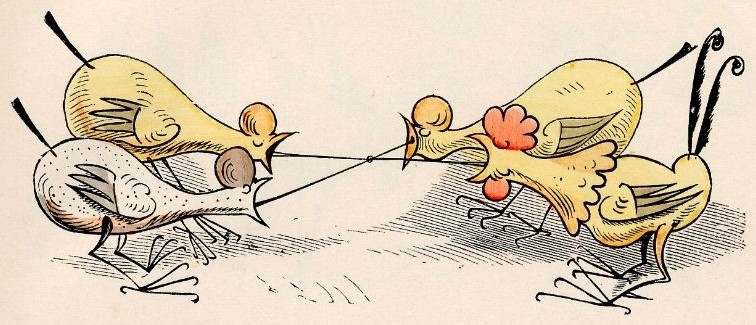
\includegraphics[scale=.7, alt={Keines kann von hinnen}]{images/1-06.jpg}\end{center}



\begin{verse}
Aber als sie sich besinnen,\\{}
Konnte keines recht von hinnen.
\end{verse}



\begin{center}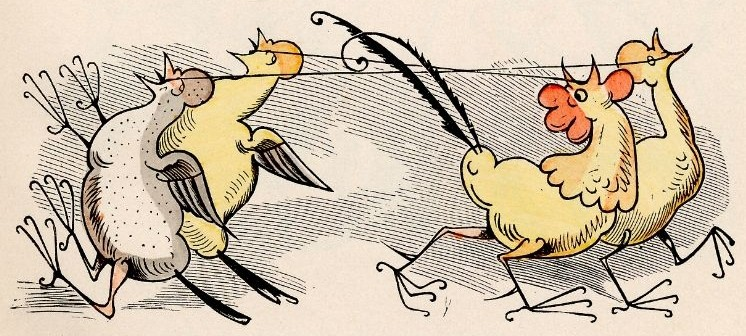
\includegraphics[scale=.7, alt={Kreuz und Quer}]{images/1-07.jpg}\end{center}



\begin{verse}
In die Kreuz und in die Quer\\{}
Reißen sie sich hin und her,
\end{verse}



\begin{center}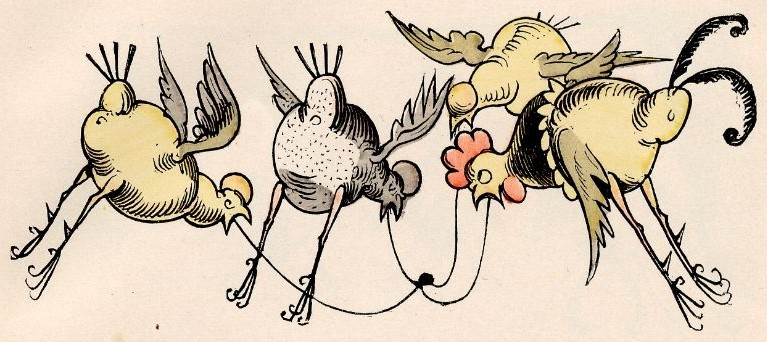
\includegraphics[scale=.7, alt={... und in die Höh}]{images/1-08.jpg}\end{center}



\begin{verse}
Flattern auf und in die Höh',\\{}
Ach herje, herjemineh!
\end{verse}



\begin{center}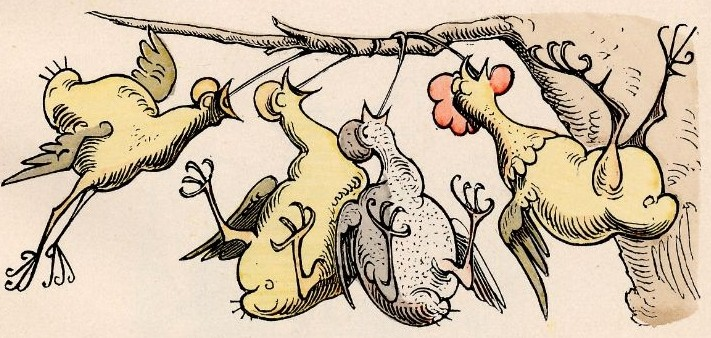
\includegraphics[scale=.7, alt={... auf den Ast}]{images/1-09.jpg}\end{center}



\begin{verse}
Ach, sie bleiben an dem langen,\\{}
Dürren Ast des Baumes hangen.~—\\{}
— Und ihr Hals wird lang und länger,\\{}
Ihr Gesang wird bang und bänger.
\end{verse}



\begin{center}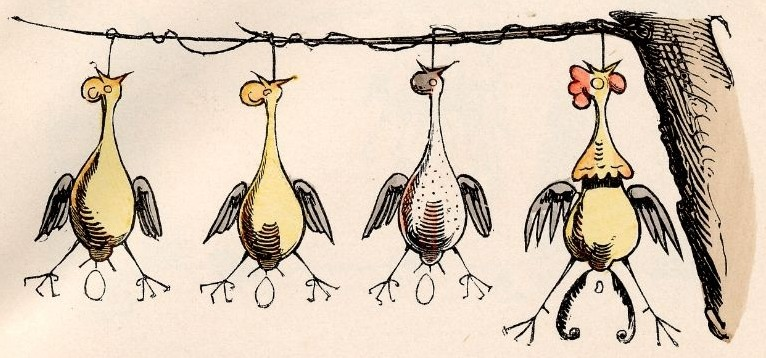
\includegraphics[scale=.7, alt={noch schnell ein Ei}]{images/1-10.jpg}\end{center}



\begin{verse}
Jedes legt noch schnell ein Ei,\\{}
Und dann kommt der Tod herbei.~—
\end{verse}



\begin{center}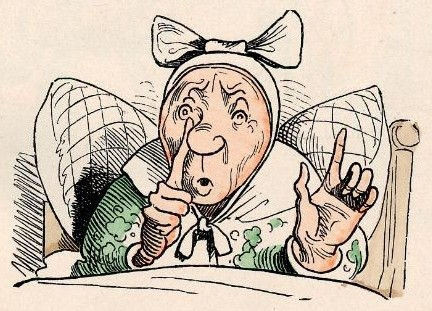
\includegraphics[scale=.7, alt={Witwe Bolte in der Kammer}]{images/1-11.jpg}\end{center}



\begin{verse}
Witwe Bolte in der Kammer\\{}
Hört im Bette diesen Jammer:
\end{verse}



\begin{center}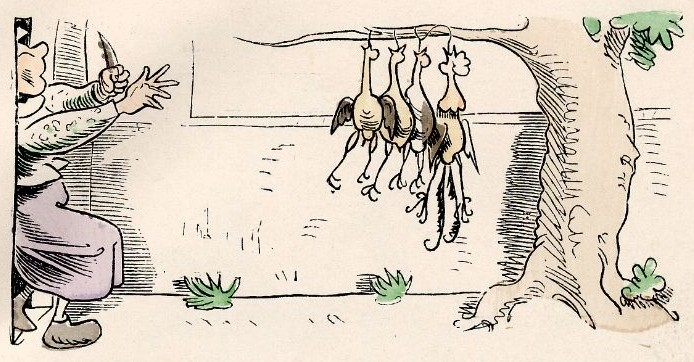
\includegraphics[scale=.7, alt={... tritt heraus}]{images/1-12.jpg}\end{center}



\begin{verse}
Ahnungsvoll tritt sie heraus,\\{}
Ach, was war das für ein Graus!
\end{verse}



\begin{center}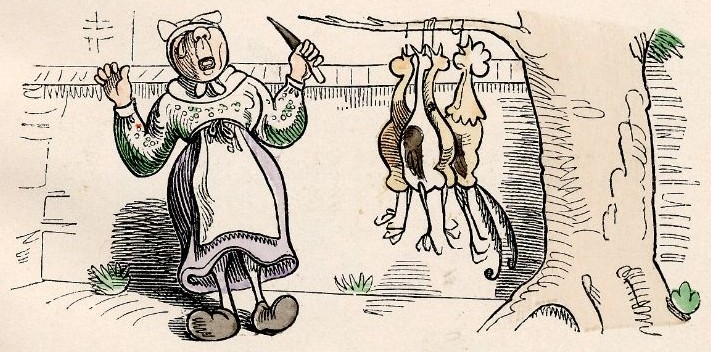
\includegraphics[scale=.7, alt={... und trauert}]{images/1-13.jpg}\end{center}



\begin{verse}
»Fließet aus dem Aug', ihr Tränen!\\{}
All' mein Hoffen, all' mein Sehnen,\\{}
Meines Lebens schönster Traum\\{}
Hängt an diesem Apfelbaum!«
\end{verse}



\begin{center}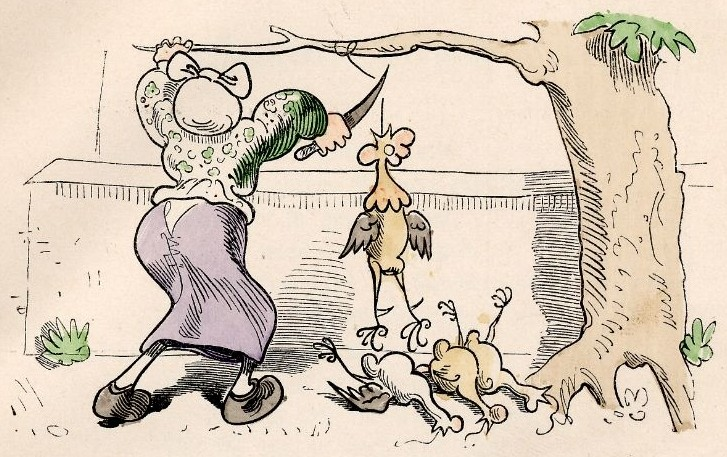
\includegraphics[scale=.7, alt={nimmt die Toten ab}]{images/1-14.jpg}\end{center}



\begin{verse}
Tiefbetrübt und sorgenschwer\\{}
Kriegt sie jetzt das Messer her,\\{}
Nimmt die Toten von den Strängen,\\{}
Daß sie so nicht länger hängen,
\end{verse}



\begin{center}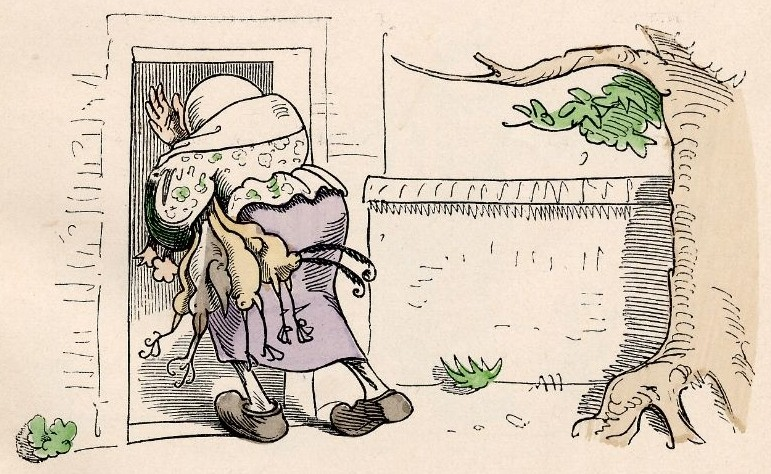
\includegraphics[scale=.7, alt={und kehrt zurück}]{images/1-15.jpg}\end{center}



\begin{verse}
Und mit stummem Trauerblick\\{}
Kehrt sie in ihr Haus zurück.
\end{verse}


\hrule


\begin{verse}
Dieses war der erste Streich,\\{}
Doch der zweite folgt sogleich.
\end{verse}


\hrule


\clearpage
\section{Zweiter Streich.\label{Zweiter_Streich}}


\begin{verse}
Als die gute Witwe Bolte\\{}
Sich von ihrem Schmerz erholte,\\{}
Dachte sie so hin und her,\\{}
Daß es wohl das beste wär',\\{}
Die Verstorb'nen, die hienieden\\{}
Schon so frühe abgeschieden,\\{}
Ganz im stillen und in Ehren\\{}
Gut gebraten zu verzehren.~—\\{}
— Freilich war die Trauer groß,\\{}
Als sie nun so nackt und bloß\\{}
Abgerupft am Herde lagen,\\{}
Sie, die einst in schönen Tagen\\{}
Bald im Hofe, bald im Garten\\{}
Lebensfroh im Sande scharrten.~—
\end{verse}



\begin{center}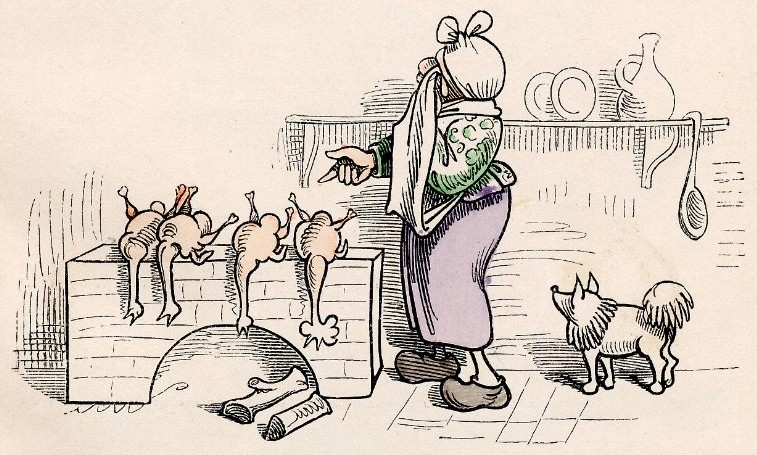
\includegraphics[scale=.7, alt={sie weint aufs neu}]{images/2-01.jpg}\end{center}



\begin{verse}
Ach, Frau Bolte weint aufs neu,\\{}
Und der Spitz steht auch dabei.\\{}
Max und Moritz rochen dieses;\\{}
»Schnell aufs Dach gekrochen!« hieß es.
\end{verse}



\begin{center}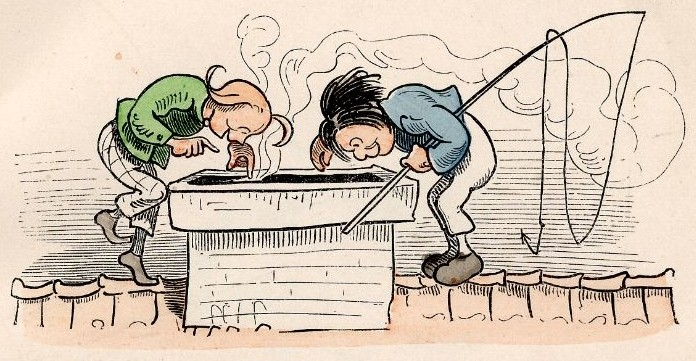
\includegraphics[scale=.7, alt={Max und Moritz auf dem Dach}]{images/2-02.jpg}\end{center}



\begin{verse}
Durch den Schornstein mit Vergnügen\\{}
Sehen sie die Hühner liegen,\\{}
Die schon ohne Kopf und Gurgeln\\{}
Lieblich in der Pfanne schmurgeln.~—
\end{verse}



\begin{center}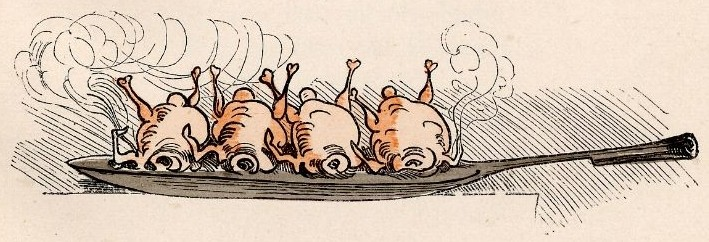
\includegraphics[scale=.7, alt={die Hühner in der Pfanne}]{images/2-03.jpg}\end{center}



\begin{verse}
Eben geht mit einem Teller\\{}
Witwe Bolte in den Keller,
\end{verse}



\begin{center}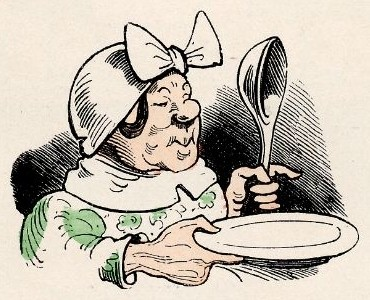
\includegraphics[scale=.7, alt={Vorfreude}]{images/2-04.jpg}\end{center}



\begin{verse}
Daß sie von dem Sauerkohle\\{}
Eine Portion sich hole,\\{}
Wofür sie besonders schwärmt,\\{}
Wenn er wieder aufgewärmt.~—\\{}
— Unterdessen auf dem Dache\\{}
Ist man tätig bei der Sache.\\{}
Max hat schon mit Vorbedacht\\{}
Eine Angel mitgebracht.
\end{verse}



\begin{center}
  \vspace*{-47pt}
  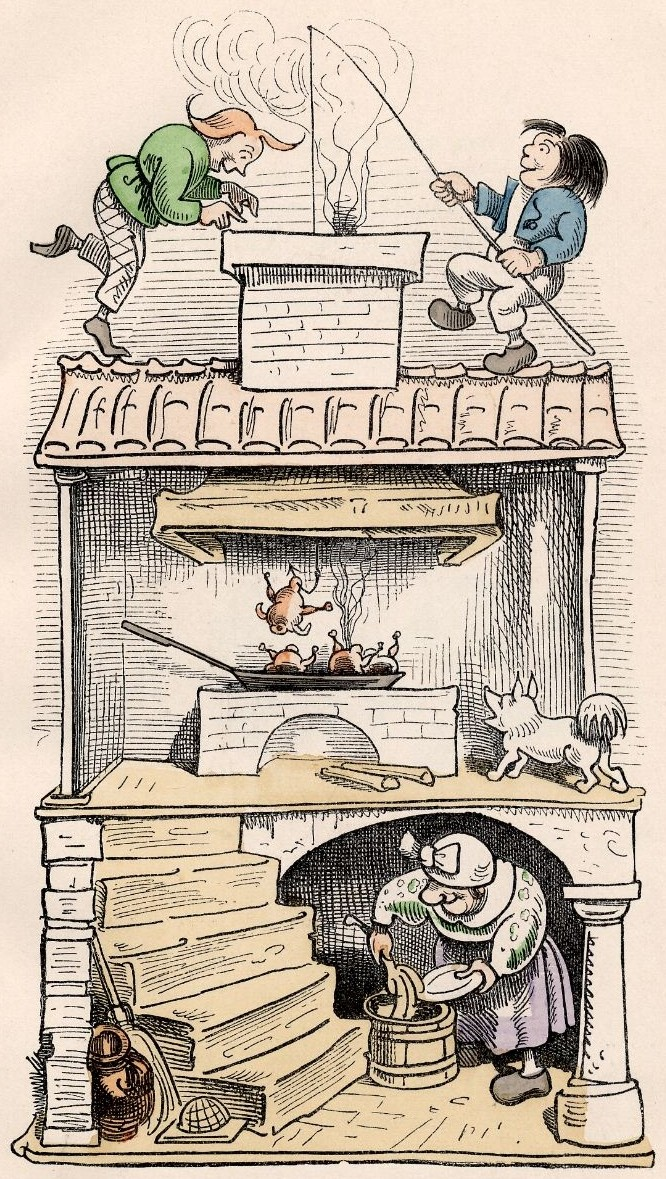
\includegraphics[scale=.7, alt={Im Haus tut sich was}]{images/2-05.jpg}
\end{center}



\begin{verse}
Schnupdiwup! da wird nach oben\\{}
Schon ein Huhn heraufgehoben;\\{}
Schnupdiwup! Jetzt Numro zwei;\\{}
Schnupdiwup! Jetzt Numro drei;\\{}
Und jetzt kommt noch Numro vier:\\{}
Schnupdiwup! Dich haben wir!~—\\{}
— Zwar der Spitz sah es genau,\\{}
Und er bellt: Rawau! Rawau!
\end{verse}



\begin{center}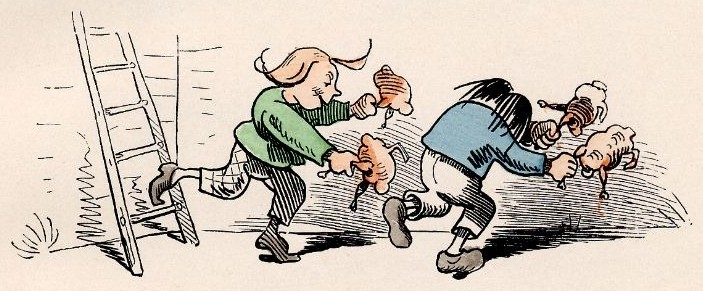
\includegraphics[scale=.7, alt={Flucht mit der Beute}]{images/2-06.jpg}\end{center}



\begin{verse}
Aber schon sind sie ganz munter\\{}
Fort und von dem Dach herunter.~—\\{}
— Na! Das wird Spektakel geben,\\{}
Denn Frau Bolte kommt soeben;~—\\{}
— Angewurzelt stand sie da,\\{}
Als sie nach der Pfanne sah.
\end{verse}



\begin{center}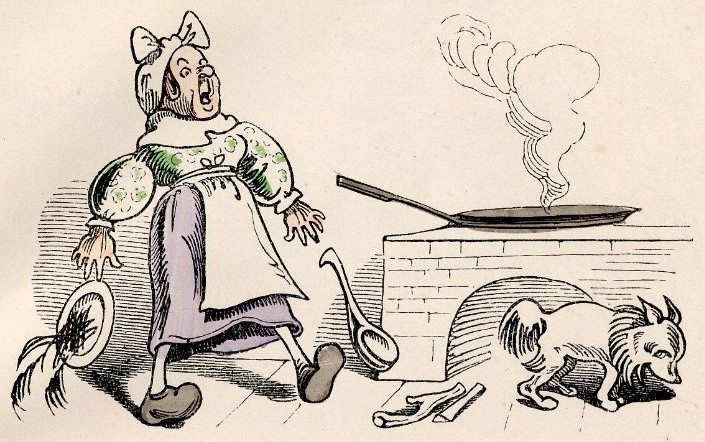
\includegraphics[scale=.7, alt={Alle Hühner waren fort}]{images/2-07.jpg}\end{center}



\begin{verse}
Alle Hühner waren fort,\\{}
»Spitz!«~— Das war ihr erstes Wort.
\end{verse}



\begin{center}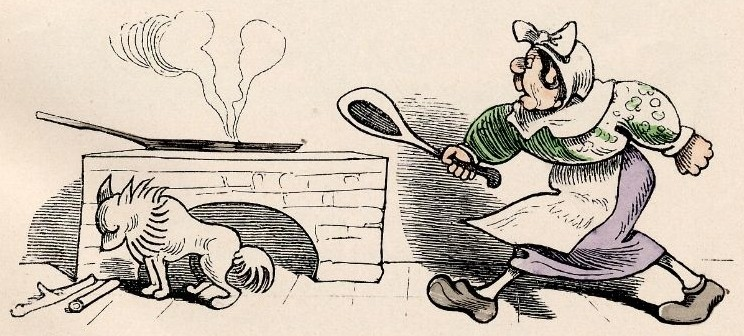
\includegraphics[scale=.7, alt={Spitz?}]{images/2-08.jpg}\end{center}



\begin{verse}
»Oh, du Spitz, du Ungetüm!\\{}
Aber wart! ich komme ihm!«
\end{verse}



\begin{center}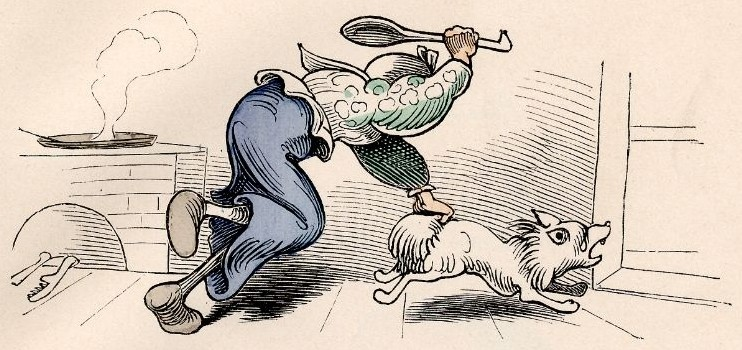
\includegraphics[scale=.7, alt={Spitz!}]{images/2-09.jpg}\end{center}



\begin{verse}
Mit dem Löffel, groß und schwer,\\{}
Geht es über Spitzen her;\\{}
Laut ertönt sein Wehgeschrei,\\{}
Denn er fühlt sich schuldenfrei.
\end{verse}



\begin{center}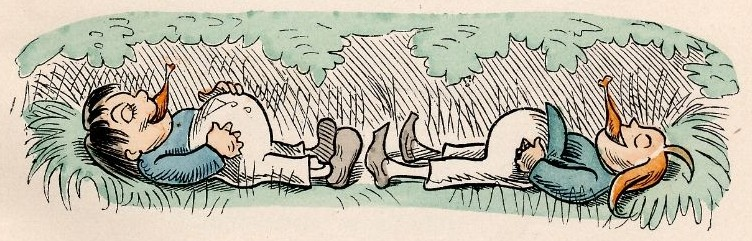
\includegraphics[scale=.7, alt={Max und Moritz im Verstecke}]{images/2-10.jpg}\end{center}



\begin{verse}
Max und Moritz im Verstecke\\{}
Schnarchen aber an der Hecke,\\{}
Und vom ganzen Hühnerschmaus\\{}
Guckt nur noch ein Bein heraus.
\end{verse}


\hrule


\begin{verse}
Dieses war der zweite Streich,\\{}
Doch der dritte folgt sogleich.
\end{verse}


\hrule


\clearpage
\section{Dritter Streich.\label{Dritter_Streich}}


\begin{verse}
Jedermann im Dorfe kannte\\{}
Einen, der sich Böck benannte.
\end{verse}



\begin{center}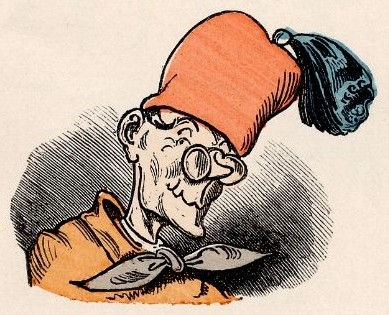
\includegraphics[scale=.7, alt={Meister Böck}]{images/3-01.jpg}\end{center}



\begin{verse}
Alltagsröcke, Sonntagsröcke,\\{}
Lange Hosen, spitze Fräcke,\\{}
Westen mit bequemen Taschen,\\{}
Warme Mäntel und Gamaschen~—\\{}
Alle diese Kleidungssachen\\{}
Wußte Schneider Böck zu machen.~—\\{}
Oder wäre was zu flicken,\\{}
Abzuschneiden, anzustücken,\\{}
Oder gar ein Knopf der Hose\\{}
Abgerissen oder lose~—\\{}
Wie und wo und wann es sei,\\{}
Hinten, vorne, einerlei~—\\{}
Alles macht der Meister Böck,\\{}
Denn das ist sein Lebenszweck.\\{}
D'rum so hat in der Gemeinde\\{}
Jedermann ihn gern zum Freunde.~—\\{}
— Aber Max und Moritz dachten,\\{}
Wie sie ihn verdrießlich machten.\\{}
Nämlich vor des Meisters Hause\\{}
Floß ein Wasser mit Gebrause.
\end{verse}



\begin{center}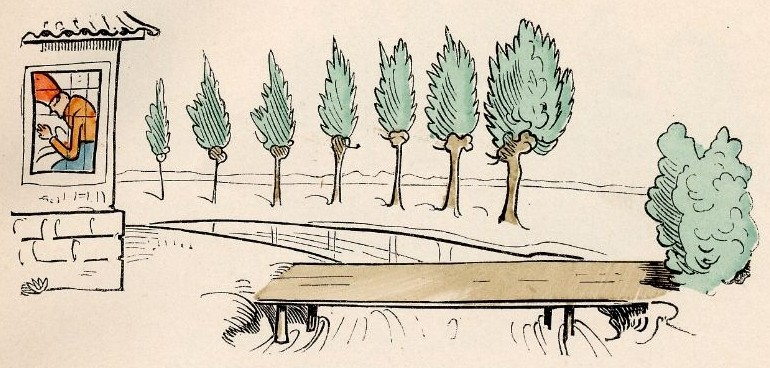
\includegraphics[scale=.7, alt={Die Brücke}]{images/3-02.jpg}\end{center}



\begin{verse}
Übers Wasser führt ein Steg\\{}
Und darüber geht der Weg.
\end{verse}



\begin{center}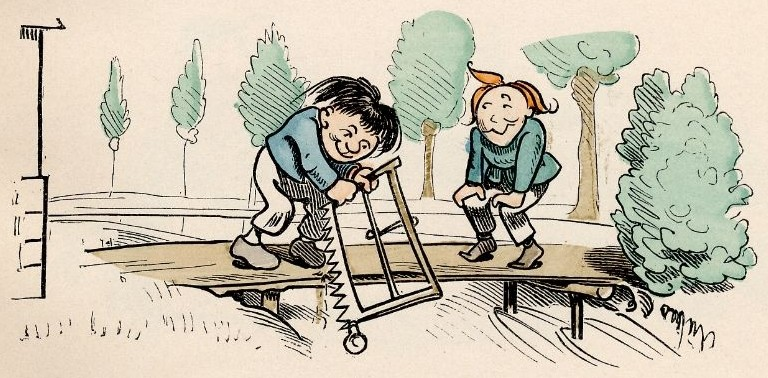
\includegraphics[scale=.7, alt={... und die Säge}]{images/3-03.jpg}\end{center}



\begin{verse}
Max und Moritz, gar nicht träge,\\{}
Sägen heimlich mit der Säge,\\{}
Ritzeratze! voller Tücke,\\{}
In die Brücke eine Lücke.\\{}
Als nun diese Tat vorbei,\\{}
Hört man plötzlich ein Geschrei:
\end{verse}



\begin{center}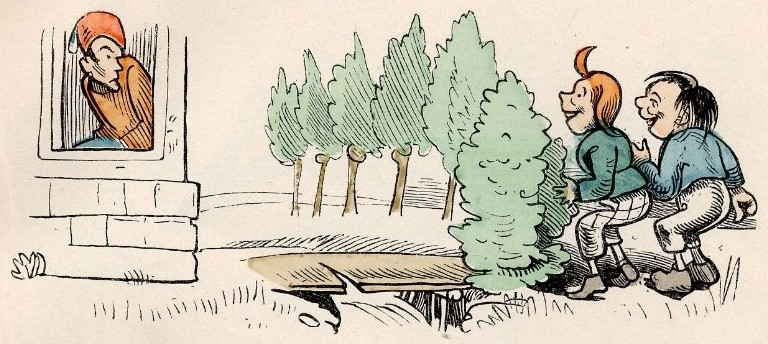
\includegraphics[scale=.7, alt={He! Heraus!}]{images/3-04.jpg}\end{center}



\begin{verse}
»He, heraus! du Ziegen-Böck!\\{}
Schneider, Schneider, meck, meck, meck!«~—\\{}
— Alles konnte Böck ertragen,\\{}
Ohne nur ein Wort zu sagen;\\{}
Aber, wenn er dies erfuhr,\\{}
Ging's ihm wider die Natur.
\end{verse}



\begin{center}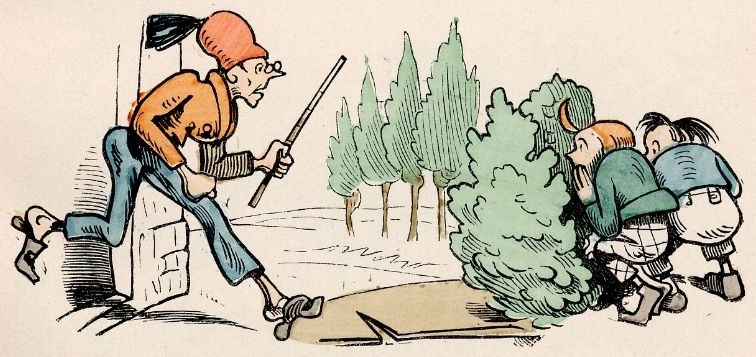
\includegraphics[scale=.7, alt={Böck kommt}]{images/3-05.jpg}\end{center}



\begin{verse}
Schnelle springt er mit der Elle\\{}
Über seines Hauses Schwelle,\\{}
Denn schon wieder ihm zum Schreck\\{}
Tönt ein lautes: »Meck, meck, meck!«
\end{verse}



\begin{center}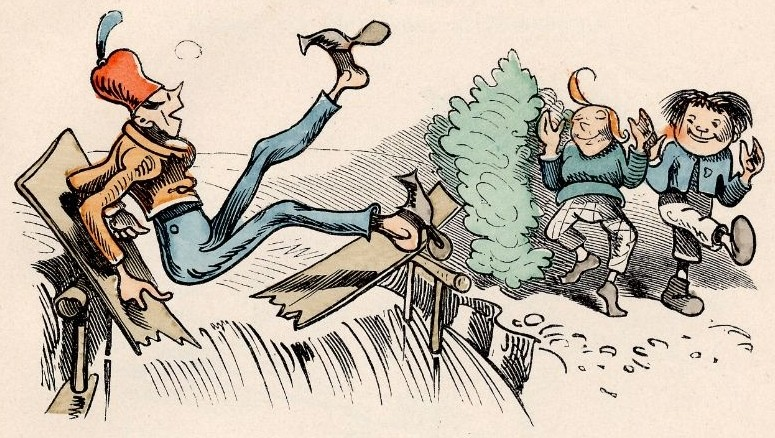
\includegraphics[scale=.7, alt={... die Brücke bricht}]{images/3-06.jpg}\end{center}



\begin{verse}
Und schon ist er auf der Brücke,\\{}
Kracks! Die Brücke bricht in Stücke;
\end{verse}



\begin{center}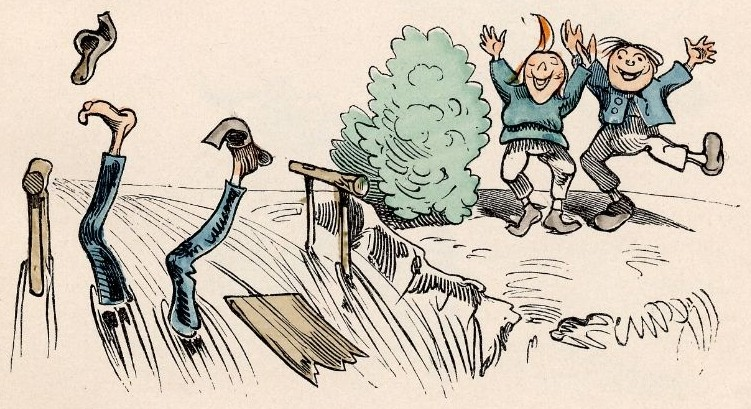
\includegraphics[scale=.7, alt={... und dann ist er weg}]{images/3-07.jpg}\end{center}



\begin{verse}
Wieder tönt es: »Meck, meck, meck!«\\{}
Plumps! Da ist der Schneider weg!\\{}
G'rad als dieses vorgekommen,\\{}
Kommt ein Gänsepaar geschwommen,
\end{verse}



\begin{center}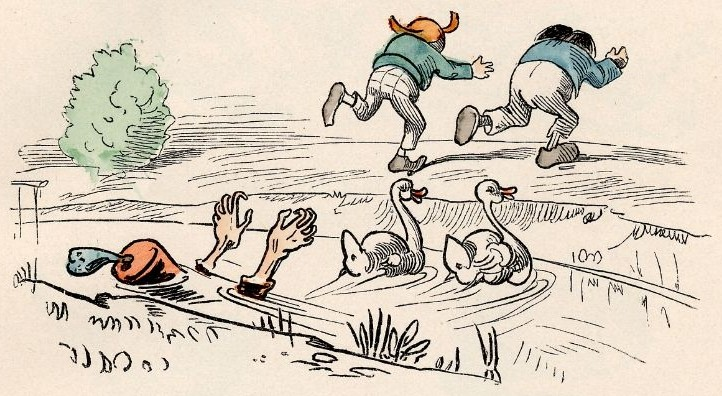
\includegraphics[scale=.7, alt={Mit den Gänsen}]{images/3-08.jpg}\end{center}



\begin{verse}
Welches Böck in Todeshast\\{}
Krampfhaft bei den Beinen faßt.
\end{verse}



\begin{center}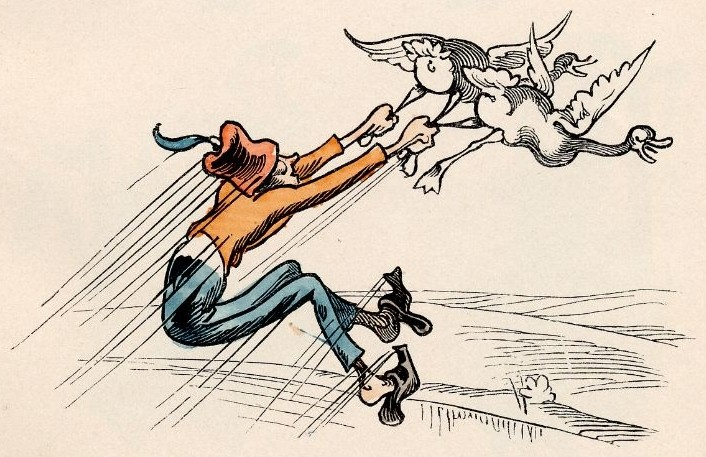
\includegraphics[scale=.7, alt={... flattert er an Land}]{images/3-09.jpg}\end{center}



\begin{verse}
Beide Gänse in der Hand,\\{}
Flattert er auf trocknes Land.
\end{verse}



\begin{center}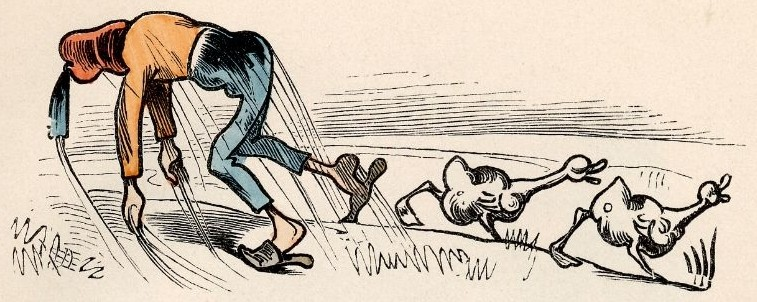
\includegraphics[scale=.7, alt={nass}]{images/3-10.jpg}\end{center}



\begin{verse}
Übrigens bei alle dem\\{}
Ist so etwas nicht bequem!
\end{verse}



\begin{center}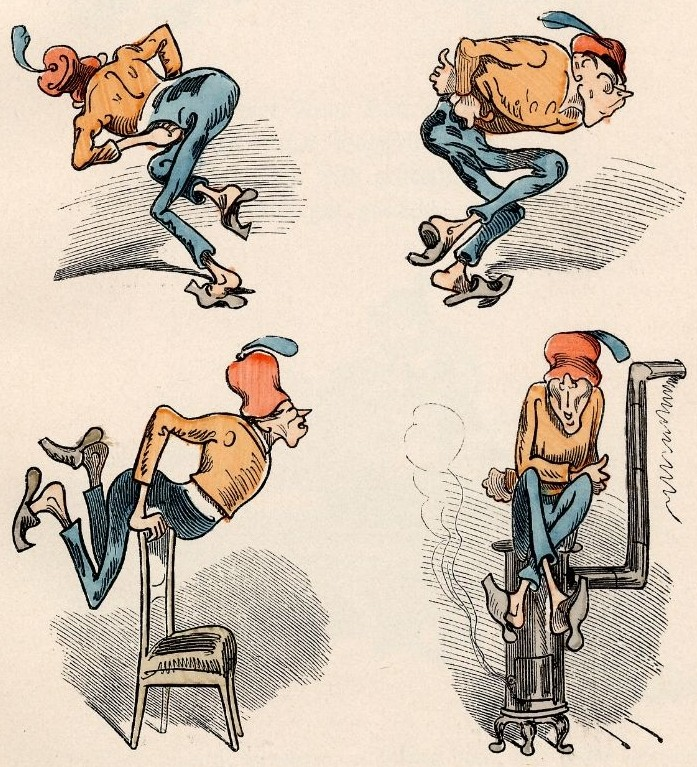
\includegraphics[scale=.7, alt={... und mit Magendrücken}]{images/3-11.jpg}\end{center}



\begin{verse}
Wie denn Böck von der Geschichte\\{}
Auch das Magendrücken kriegte.
\end{verse}



\begin{center}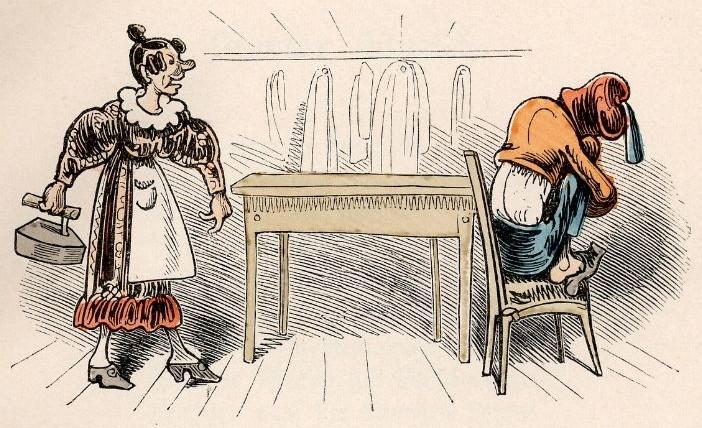
\includegraphics[scale=.7, alt={Frau Böck}]{images/3-12.jpg}\end{center}



\begin{verse}
Hoch ist hier Frau Böck zu preisen!\\{}
Denn ein heißes Bügeleisen,\\{}
Auf den kalten Leib gebracht,\\{}
Hat es wieder gut gemacht.
\end{verse}



\begin{center}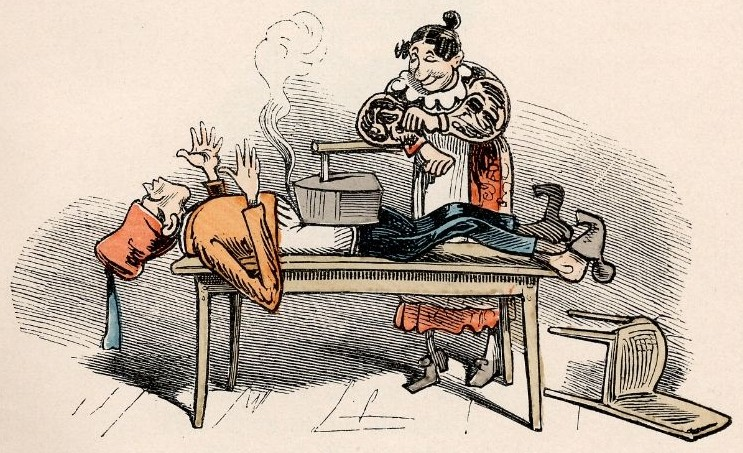
\includegraphics[scale=.7, alt={... mit dem Bügeleisen}]{images/3-13.jpg}\end{center}



\begin{verse}
— Bald im Dorf hinauf, hinunter,\\{}
Hieß es, Böck ist wieder munter.
\end{verse}


\hrule


\begin{verse}
Dieses war der dritte Streich,\\{}
Doch der vierte folgt sogleich.
\end{verse}


\hrule


\clearpage
\section{Vierter Streich.\label{Vierter_Streich}}


\begin{verse}
Also lautet ein Beschluß:\\{}
Daß der Mensch was lernen muß.~—\\{}
Nicht allein das A-B-C\\{}
Bringt den Menschen in die Höh';\\{}
Nicht allein im Schreiben, Lesen\\{}
Übt sich ein vernünftig Wesen;\\{}
Nicht allein in Rechnungssachen\\{}
Soll der Mensch sich Mühe machen;\\{}
Sondern auch der Weisheit Lehren\\{}
Muß man mit Vergnügen hören.
\end{verse}



\begin{center}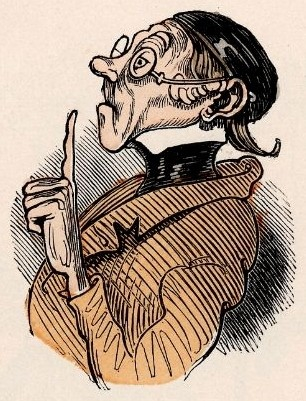
\includegraphics[scale=.7, alt={Lehrer Lämpel}]{images/4-01.jpg}\end{center}



\begin{verse}
Daß dies mit Verstand geschah,\\{}
War Herr Lehrer Lämpel da.~—\\{}
— Max und Moritz, diese beiden,\\{}
Mochten ihn darum nicht leiden;\\{}
Denn wer böse Streiche macht,\\{}
Gibt nicht auf den Lehrer acht.\\{}
Nun war dieser brave Lehrer\\{}
Von dem Tobak ein Verehrer,\\{}
Was man ohne alle Frage\\{}
Nach des Tages Müh und Plage\\{}
Einem guten, alten Mann\\{}
Auch von Herzen gönnen kann.~—\\{}
— Max und Moritz, unverdrossen,\\{}
Sinnen aber schon auf Possen,\\{}
Ob vermittelst seiner Pfeifen\\{}
Dieser Mann nicht anzugreifen.~—\\{}
— Einstens, als es Sonntag wieder\\{}
Und Herr Lämpel brav und bieder
\end{verse}



\begin{center}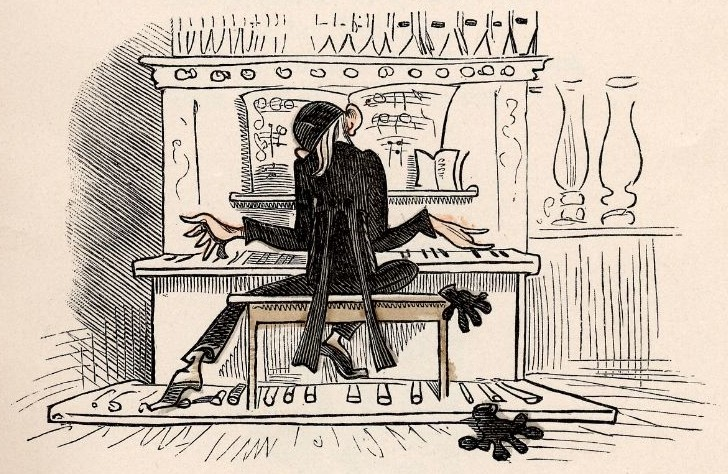
\includegraphics[scale=.7, alt={an der Orgel}]{images/4-02.jpg}\end{center}



\begin{verse}
In der Kirche mit Gefühle\\{}
Saß vor seinem Orgelspiele,\\{}
Schlichen sich die bösen Buben\\{}
In sein Haus und seine Stuben,\\{}
Wo die Meerschaumpfeife stand;\\{}
Max hält sie in seiner Hand;
\end{verse}



\begin{center}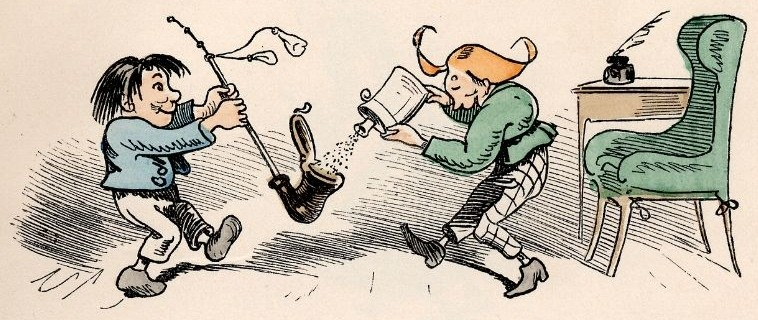
\includegraphics[scale=.7, alt={Max und Moritz mit der Pulverflasche}]{images/4-03.jpg}\end{center}



\begin{verse}
Aber Moritz aus der Tasche\\{}
Zieht die Flintenpulverflasche,\\{}
Und geschwinde, stopf, stopf, stopf!\\{}
Pulver in den Pfeifenkopf.~—\\{}
Jetzt nur still und schnell nach Haus,\\{}
Denn schon ist die Kirche aus.~—
\end{verse}



\begin{center}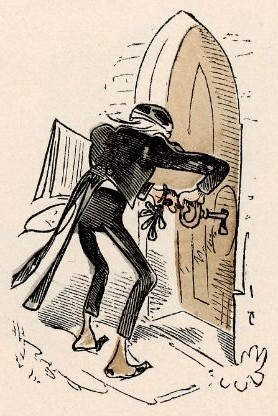
\includegraphics[scale=.7, alt={an der Kirchentür}]{images/4-04.jpg}\end{center}



\begin{verse}
Eben schließt in sanfter Ruh'\\{}
Lämpel seine Kirche zu;\\{}
Und mit Buch und Notenheften,\\{}
Nach besorgten Amtsgeschäften,
\end{verse}



\begin{center}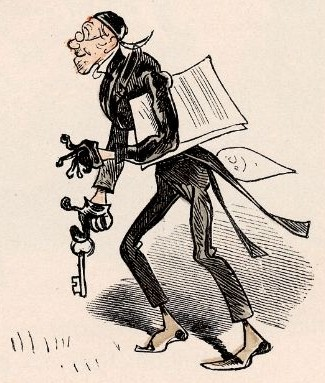
\includegraphics[scale=.7, alt={am Nachhauseweg}]{images/4-05.jpg}\end{center}



\begin{verse}
Lenkt er freudig seine Schritte\\{}
Zu der heimatlichen Hütte,
\end{verse}



\begin{center}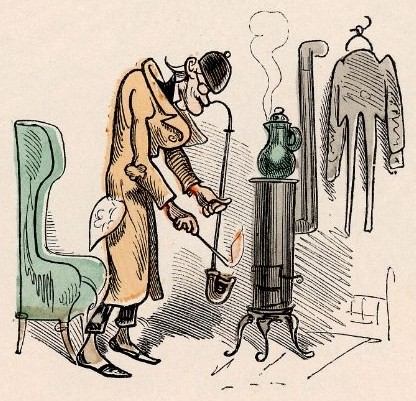
\includegraphics[scale=.7, alt={die Pfeife wird angezündet}]{images/4-06.jpg}\end{center}



\begin{verse}
Und voll Dankbarkeit sodann,\\{}
Zündet er sein Pfeifchen an.
\end{verse}



\begin{center}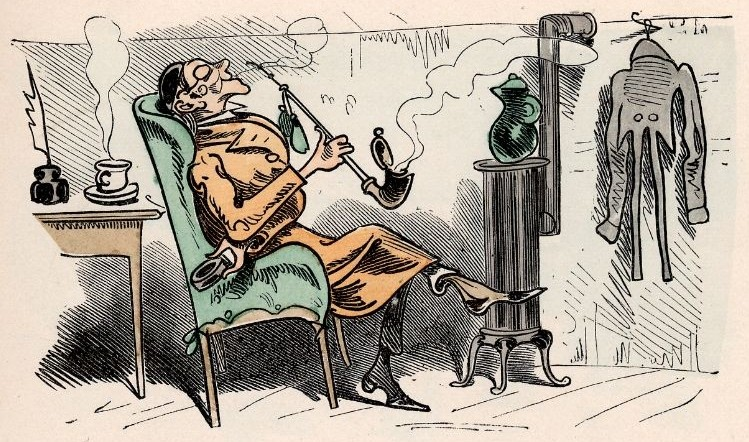
\includegraphics[scale=.7, alt={... und man ist zufrieden}]{images/4-07.jpg}\end{center}



\begin{verse}
»Ach!«~— spricht er~— »die größte Freud'\\{}
Ist doch die Zufriedenheit!«
\end{verse}



\begin{center}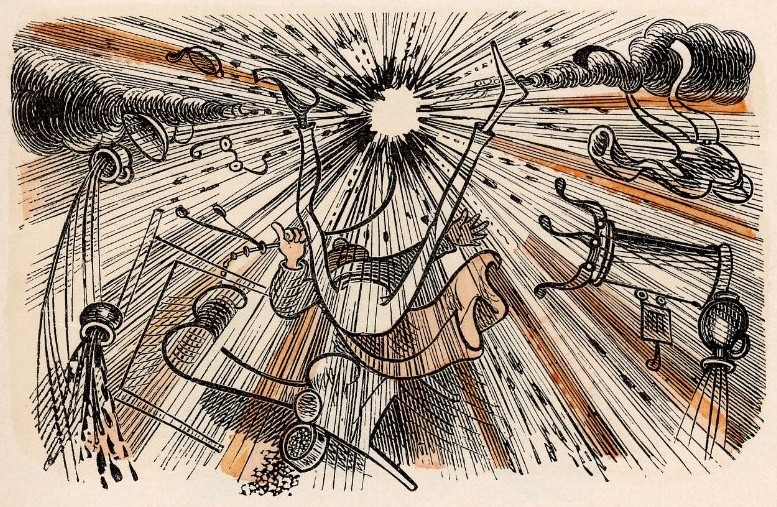
\includegraphics[scale=.7, alt={Rums!}]{images/4-08.jpg}\end{center}



\begin{verse}
Rums! Da geht die Pfeife los\\{}
Mit Getöse, schrecklich groß.\\{}
Kaffeetopf und Wasserglas,\\{}
Tabaksdose, Tintenfaß,\\{}
Ofen, Tisch und Sorgensitz~—\\{}
Alles fliegt im Pulverblitz.
\end{verse}



\begin{center}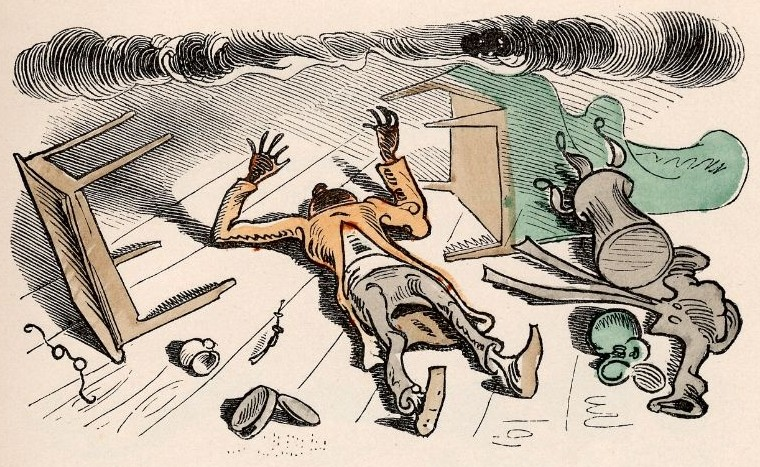
\includegraphics[scale=.7, alt={Lebend auf dem Rücken}]{images/4-09.jpg}\end{center}



\begin{verse}
Als der Dampf sich nun erhob,\\{}
Sieht man Lämpel, der gottlob!\\{}
Lebend auf dem Rücken liegt;\\{}
Doch er hat was abgekriegt.
\end{verse}



\begin{center}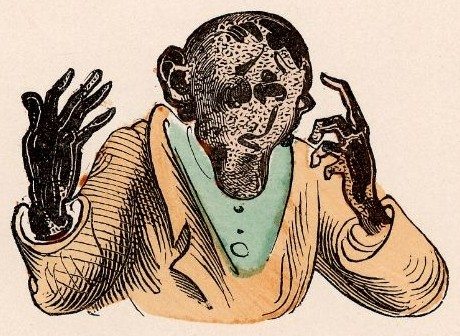
\includegraphics[scale=.7, alt={schwarz wie ein Mohr}]{images/4-10.jpg}\end{center}



\begin{verse}
Nase, Hand, Gesicht und Ohren\\{}
Sind so schwarz als wie die Mohren,\\{}
Und des Haares letzter Schopf\\{}
Ist verbrannt bis auf den Kopf.\\{}
Wer soll nun die Kinder lehren\\{}
Und die Wissenschaft vermehren?\\{}
Wer soll nun für Lämpel leiten\\{}
Seine Amtestätigkeiten?\\{}
Woraus soll der Lehrer rauchen,\\{}
Wenn die Pfeife nicht zu brauchen?
\end{verse}



\begin{center}\includegraphics[scale=.7, alt={die Pfeife hat ihr Teil}]{images/4-11.jpg}\end{center}



\begin{verse}
Mit der Zeit wird alles heil,\\{}
Nur die Pfeife hat ihr Teil.
\end{verse}


\hrule


\begin{verse}
Dieses war der vierte Streich,\\{}
Doch der fünfte folgt sogleich.
\end{verse}


\hrule


\clearpage
\section{Fünfter Streich.\label{Funfter_Streich}}


\begin{verse}
Wer im Dorfe oder Stadt\\{}
Einen Onkel wohnen hat,\\{}
Der sei höflich und bescheiden,\\{}
Denn das mag der Onkel leiden.~—\\{}
— Morgens sagt man: »Guten Morgen!\\{}
Haben Sie was zu besorgen?«\\{}
Bringt ihm, was er haben muß:\\{}
Zeitung, Pfeife, Fidibus.~—\\{}
Oder sollt' es wo im Rücken\\{}
Drücken, beißen oder zwicken,\\{}
Gleich ist man mit Freudigkeit\\{}
Dienstbeflissen und bereit.~—\\{}
Oder sei's nach einer Prise,\\{}
Daß der Onkel heftig niese,\\{}
Ruft man: »Prosit!« allsogleich,\\{}
»Danke,« — »wohl bekomm' es euch!«~—\\{}
Oder kommt er spät nach Haus,\\{}
Zieht man ihm die Stiefel aus,\\{}
Holt Pantoffel, Schlafrock, Mütze,\\{}
Daß er nicht im Kalten sitze,~—\\{}
Kurz, man ist darauf bedacht,\\{}
Was dem Onkel Freude macht.~—\\{}
— Max und Moritz ihrerseits\\{}
Fanden darin keinen Reiz.~—\\{}
— Denkt euch nur, welch' schlechten Witz\\{}
Machten sie mit Onkel Fritz!\\{}
Jeder weiß, was so ein Mai–\\{}
Käfer für ein Vogel sei.
\end{verse}



\begin{center}\includegraphics[scale=.7, alt={Maikäfer}]{images/5-01.jpg}\end{center}



\begin{verse}
In den Bäumen hin und her\\{}
Fliegt und kriecht und krabbelt er.
\end{verse}



\begin{center}\includegraphics[scale=.7, alt={... schütteln}]{images/5-02.jpg}\end{center}



\begin{verse}
Max und Moritz, immer munter,\\{}
Schütteln sie vom Baum herunter.
\end{verse}



\begin{center}\includegraphics[scale=.7, alt={... und in die Tüte}]{images/5-03.jpg}\end{center}



\begin{verse}
In die Düte von Papiere\\{}
Sperren sie die Krabbeltiere.
\end{verse}



\begin{center}\includegraphics[scale=.7, alt={Ab unter die Decke}]{images/5-04.jpg}\end{center}



\begin{verse}
Fort damit und in die Ecke\\{}
Unter Onkel Fritzens Decke!
\end{verse}



\begin{center}\includegraphics[scale=.7, alt={Onkel Fritze geht zu Bette}]{images/5-05.jpg}\end{center}



\begin{verse}
Bald zu Bett geht Onkel Fritze\\{}
In der spitzen Zippelmütze;\\{}
Seine Augen macht er zu,\\{}
Hüllt sich ein und schläft in Ruh.
\end{verse}



\begin{center}\includegraphics[scale=.7, alt={... und schläft in Ruh}]{images/5-06.jpg}\end{center}




\begin{center}\includegraphics[scale=.7, alt={Die Käfer}]{images/5-07.jpg}\end{center}



\begin{verse}
Doch die Käfer, kritze, kratze!\\{}
Kommen schnell aus der Matratze.
\end{verse}



\begin{center}\includegraphics[scale=.7, alt={... kommen}]{images/5-08.jpg}\end{center}



\begin{verse}
Schon faßt einer, der voran,\\{}
Onkel Fritzens Nase an.
\end{verse}



\begin{center}\includegraphics[scale=.7, alt={und werden erfasst}]{images/5-09.jpg}\end{center}



\begin{verse}
»Bau!« schreit er~— »Was ist das hier?«\\{}
Und erfaßt das Ungetier.
\end{verse}



\begin{center}\includegraphics[scale=.7, alt={der Onkel saust}]{images/5-10.jpg}\end{center}



\begin{verse}
Und den Onkel voller Grausen\\{}
Sieht man aus dem Bette sausen.
\end{verse}



\begin{center}\includegraphics[scale=.7, alt={... denn es kriecht}]{images/5-11.jpg}\end{center}



\begin{verse}
»Autsch!«~— Schon wieder hat er einen\\{}
Im Genicke, an den Beinen;
\end{verse}



\begin{center}\includegraphics[scale=.7, alt={... und fliegt}]{images/5-12.jpg}\end{center}



\begin{verse}
Hin und her und rund herum\\{}
Kriecht es, fliegt es mit Gebrumm.
\end{verse}



\begin{center}\includegraphics[scale=.7, alt={Onkel Fritz haut}]{images/5-13.jpg}\end{center}



\begin{verse}
Onkel Fritz, in dieser Not,\\{}
Haut und trampelt alles tot.
\end{verse}



\begin{center}\includegraphics[scale=.7, alt={... und trampelt alles tot}]{images/5-14.jpg}\end{center}



\begin{verse}
Guckste wohl! Jetzt ist's vorbei\\{}
Mit der Käferkrabbelei!
\end{verse}



\begin{center}\includegraphics[scale=.7, alt={wieder Ruhe}]{images/5-15.jpg}\end{center}



\begin{verse}
Onkel Fritz hat wieder Ruh'\\{}
Und macht seine Augen zu.
\end{verse}


\hrule


\begin{verse}
Dieses war der fünfte Streich,\\{}
Doch der sechste folgt sogleich.
\end{verse}


\hrule


\clearpage
\section{Sechster Streich.\label{Sechster_Streich}}


\begin{verse}
In der schönen Osterzeit,\\{}
Wenn die frommen Bäckersleut'\\{}
Viele süße Zuckersachen\\{}
Backen und zurechte machen,\\{}
Wünschten Max und Moritz auch\\{}
Sich so etwas zum Gebrauch.
\end{verse}



\begin{center}\includegraphics[scale=.7, alt={Der Bäcker macht das Backhaus zu}]{images/6-01.jpg}\end{center}



\begin{verse}
Doch der Bäcker, mit Bedacht,\\{}
Hat das Backhaus zugemacht.
\end{verse}



\begin{center}\includegraphics[scale=.7, alt={Durch den Schlot}]{images/6-02.jpg}\end{center}



\begin{verse}
Also will hier einer stehlen,\\{}
Muß er durch den Schlot sich quälen.
\end{verse}



\begin{center}\includegraphics[scale=.7, alt={Schwarz wie Raben}]{images/6-03.jpg}\end{center}



\begin{verse}
Ratsch! Da kommen die zwei Knaben\\{}
Durch den Schornstein, schwarz wie Raben.
\end{verse}



\begin{center}\includegraphics[scale=.7, alt={... in die Mehlkist'}]{images/6-04.jpg}\end{center}



\begin{verse}
Puff! Sie fallen in die Kist',\\{}
Wo das Mehl darinnen ist.
\end{verse}



\begin{center}\includegraphics[scale=.7, alt={Weiß wie Kreide}]{images/6-05.jpg}\end{center}



\begin{verse}
Da! Nun sind sie alle beide,\\{}
Rund herum so weiß wie Kreide.
\end{verse}



\begin{center}\includegraphics[scale=.7, alt={Auf den Stuhl}]{images/6-06.jpg}\end{center}



\begin{verse}
Aber schon mit viel Vergnügen\\{}
Sehen sie die Brezeln liegen.
\end{verse}



\begin{center}\includegraphics[scale=.7, alt={... der bricht entzwei}]{images/6-07.jpg}\end{center}



\begin{verse}
Knacks!~— Da bricht der Stuhl entzwei;
\end{verse}



\begin{center}\includegraphics[scale=.7, alt={... und in den Brei}]{images/6-08.jpg}\end{center}



\begin{verse}
Schwapp!~— Da liegen sie im Brei.
\end{verse}



\begin{center}\includegraphics[scale=.7, alt={Voll Kuchenteig}]{images/6-09.jpg}\end{center}



\begin{verse}
Ganz von Kuchenteig umhüllt,\\{}
Steh'n sie da als Jammerbild.~—
\end{verse}



\begin{center}\includegraphics[scale=.7, alt={... bemerkt sie Meister Bäcker}]{images/6-10.jpg}\end{center}



\begin{verse}
Gleich erscheint der Meister Bäcker\\{}
Und bemerkt die Zuckerlecker.
\end{verse}



\begin{center}\includegraphics[scale=.7, alt={Zwei Brote}]{images/6-11.jpg}\end{center}



\begin{verse}
Eins, zwei, drei!~— eh' man's gedacht,\\{}
Sind zwei Brote d'raus gemacht.
\end{verse}



\begin{center}\includegraphics[scale=.7, alt={... in das Ofenloch}]{images/6-12.jpg}\end{center}



\begin{verse}
In dem Ofen glüht es noch~—\\{}
Ruff!~— damit ins Ofenloch!
\end{verse}



\begin{center}\includegraphics[scale=.7, alt={... und aus der Glut}]{images/6-13.jpg}\end{center}



\begin{verse}
Ruff! man zieht sie aus der Glut;\\{}
Denn nun sind sie braun und gut.~—
\end{verse}



\begin{center}\includegraphics[scale=.7, alt={Noch leben sie}]{images/6-14.jpg}\end{center}



\begin{verse}
Jeder denkt, die sind perdü!\\{}
Aber nein~— noch leben sie.
\end{verse}



\begin{center}\includegraphics[scale=.7, alt={Knusper, Knasper}]{images/6-15.jpg}\end{center}



\begin{verse}
Knusper, Knasper!~— wie zwei Mäuse\\{}
Fressen sie durch das Gehäuse;
\end{verse}



\begin{center}\includegraphics[scale=.7, alt={Da laufen sie}]{images/6-16.jpg}\end{center}



\begin{verse}
Und der Meister Bäcker schrie:\\{}
»Ach herrjeh! da laufen sie!«
\end{verse}


\hrule


\begin{verse}
Dieses war der sechste Streich,\\{}
Doch der letzte folgt sogleich.
\end{verse}


\hrule


\clearpage
\section{Letzter Streich.\label{Letzter_Streich}}


\begin{verse}
Max und Moritz, wehe euch!\\{}
Jetzt kommt euer letzter Streich!
\end{verse}



\begin{center}\includegraphics[scale=.7, alt={Löcher in die Säcke}]{images/7-01.jpg}\end{center}



\begin{verse}
Wozu müssen auch die beiden\\{}
Löcher in die Säcke schneiden?
\end{verse}



\begin{center}\includegraphics[scale=.7, alt={Bauer Mecke}]{images/7-02.jpg}\end{center}



\begin{verse}
Seht, da trägt der Bauer Mecke\\{}
Einen seiner Maltersäcke.
\end{verse}



\begin{center}\includegraphics[scale=.7, alt={Die Säcke rinnen}]{images/7-03.jpg}\end{center}



\begin{verse}
Aber kaum, daß er von hinnen,\\{}
Fängt das Korn schon an zu rinnen.
\end{verse}



\begin{center}\includegraphics[scale=.7, alt={... und werden lichter}]{images/7-04.jpg}\end{center}



\begin{verse}
Und verwundert steht und spricht er:\\{}
»Zapperment! dat Ding werd lichter!«
\end{verse}



\begin{center}\includegraphics[scale=.7, alt={Voller Freude}]{images/7-05.jpg}\end{center}



\begin{verse}
Hei! Da sieht er voller Freude\\{}
Max und Moritz im Getreide.
\end{verse}



\begin{center}\includegraphics[scale=.7, alt={In den Sack}]{images/7-06.jpg}\end{center}



\begin{verse}
Rabs!~— in seinen großen Sack\\{}
Schaufelt er das Lumpenpack.
\end{verse}



\begin{center}\includegraphics[scale=.7, alt={... zur Mühle}]{images/7-07.jpg}\end{center}



\begin{verse}
Max und Moritz wird es schwüle,\\{}
Denn nun geht es nach der Mühle.~—
\end{verse}



\begin{center}\includegraphics[scale=.7, alt={... zu Meister Müller}]{images/7-08.jpg}\end{center}



\begin{verse}
»Meister Müller, he, heran!\\{}
Mahl er das, so schnell er kann!«
\end{verse}



\begin{center}\includegraphics[scale=.7, alt={... in den Trichter}]{images/7-09.jpg}\end{center}



\begin{verse}
»Her damit!« Und in den Trichter\\{}
Schüttelt er die Bösewichter.~—
\end{verse}



\begin{center}\includegraphics[scale=.7, alt={... und herau}]{images/7-10.jpg}\end{center}



\begin{verse}
Rickeracke! Rickeracke!\\{}
Geht die Mühle mit Geknacke.
\end{verse}



\begin{center}\includegraphics[scale=.7, alt={Fein geschroten}]{images/7-11.jpg}\end{center}



\begin{verse}
Hier kann man sie noch erblicken\\{}
Fein geschroten und in Stücken.
\end{verse}



\begin{center}\includegraphics[scale=.7, alt={... und verzehrt}]{images/7-12.jpg}\end{center}



\begin{verse}
Doch sogleich verzehret sie
\end{verse}



\begin{center}\includegraphics[scale=.7, alt={... vom Federvieh}]{images/7-13.jpg}\end{center}



\begin{verse}
Meister Müllers Federvieh.
\end{verse}


\hrule


\clearpage
\section{Schluß.\label{Schluss}}


\begin{verse}
Als man dies im Dorf erfuhr,\\{}
War von Trauer keine Spur.~—\\{}
— Witwe Bolte, mild und weich,\\{}
Sprach: »Sieh' da, ich dacht' es gleich!«~—\\{}
— »Ja, ja, ja!« rief Meister Böck,\\{}
»Bosheit ist kein Lebenszweck!«\\{}
— Drauf so sprach Herr Lehrer Lämpel:\\{}
»Dies ist wieder ein Exempel!«~—\\{}
— »Freilich!« meint der Zuckerbäcker,\\{}
»Warum ist der Mensch so lecker!«~—\\{}
— Selbst der gute Onkel Fritze\\{}
Sprach: »Das kommt von dumme Witze!«~—\\{}
— Doch der brave Bauersmann\\{}
Dachte: »Wat geiht meck dat an!«~—\\{}
— Kurz im ganzen Ort herum\\{}
Ging ein freudiges Gebrumm:\\{}
»Gott sei Dank! Nun ist's vorbei\\{}
Mit der Übeltäterei!!«
\end{verse}


\begin{verbatim}

\end{verbatim}


\clearpage

    
\begin{otherlanguage}{english}

\section*{The Project Gutenberg License\label{pg-license}}

\begin{center}
The source material for this edition was obtained from\\
\href{https://gutenberg.org/ebooks/17161}{\textbf{The Project Gutenberg}}
under the
\href{https://www.gutenberg.org/policy/license.html}{\textbf{Project Gutenberg License}}.
\end{center}



    
\end{otherlanguage}


  \end{document}
  
 
